\chapter{User Manual}

\minitoc

\section{Introduction}

This user manual will explain how to use the system that has been created
for you, the user.  If anything is not clear, please contact me, or attempt
to work the functioning out!  My contact details are provided in a separate,
user-only document.

\section{Usage instructions}
	\subsection{Installing the program}

The first step is the installation of the program!  To do this, navigate to
the folder view of the USB stick that the program will be provided on, and
click setup.  A window like this will display:

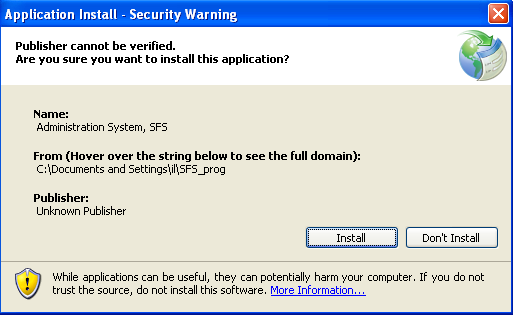
\includegraphics[scale=0.5]{um_installoptionwarning}

Click Install, ignoring any warnings about untrusted publishers.  The
program will then install reasonably quickly.

	\subsection{Launching the program}

To use the program, click Start, then the below:


\includegraphics[scale=0.5]{um_startmenu}

 	\subsection{Logging in}
	When the program has successfully launched, the login form will display.  This form demands a username and password: any of the ones provided in the table below may be used.  Enter the username in the username textbox indicated, and the password into the password textbox, then click on or tab to the OK button.

	\begin{longtable} { | p{2cm} | p{2cm} | }
		\hline
		\textbf{Username} & \textbf{Password}\\
		\endfirsthead		
		\hline
		\textbf{Username (cont.)} & \textbf{Password (cont.)}\\
		\endhead
		\hline
		sfs & sfs\\
		\hline
	\end{longtable}

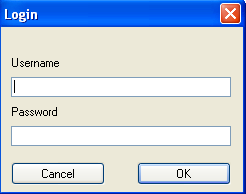
\includegraphics[scale=0.5]{frmLoginForm_scrot}
	
	If the login attempt is unsuccessful, an error message box will display.  Try entering the details again.  If the error persists, contact me---it may be due to a typo in the database or this document.
	
	If everything is fine, either on the first, second, or $n$th attempt, the login form should hide itself and the main menu should appear.
	
	\subsection{The main menu}	
	The main menu is the core from which everything can be accessed.
	
	The menu, as below, contains buttons that can be clicked to access various parts of the program.  This manual will explain each of them in turn.
	
	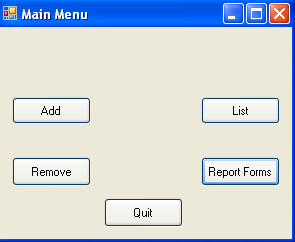
\includegraphics[scale=0.5]{frmMainMenu_scrot}

	\subsection{Adding customers, suppliers, or components}
	
	Clicking the add button from the main menu will open the Add form, where it is possibe to select what to add: either customer, supplier, or component, as below.
	
	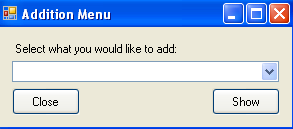
\includegraphics[scale=0.5]{frmAdd_scrot}
	
	Click on the dropdown box to select either Customer, Supplier, or Component, then click OK.  The appropriate form will display.  Read on\ldots.
	
		\subsubsection{Customers}
		
		If Customers is chosen, the add customer form appears:.
		
		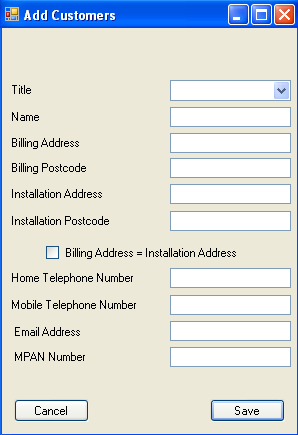
\includegraphics[scale=0.5]{frmAddCustomer_scrot}
		
		Input the details, then click Save.  If there is an error in the details, the program will give an error message and data amendment is possible.  If there is no error and therefore the data insertion is successful, the save textbox will turn grey, signifying that the form can be closed safely.  
		
		Clicking the Cancel button will close the form, thereby not saving any of the data entered into the textboxes.

		Some things to note:
		
		\begin{itemize}
			\item{If there is no data to input into one textbox at the time of addition, input `NULL', do not just leave the textbox blank: doing so will display an error.}
			\item{The customer name must be in the format \textsl{Forename Surname}---there are not separate textboxes for forename and surname.}
			\item{UK telephone numbers must contain spaces between them, e.g. \textsl{01234 567890}, \textsc{NOT} \textsl{01234567890} or variants.}
			\item{If the customer's installation address is the same as their already entered billing address, tick the box: this will automatically populate the installation address fields in the form and the database.}
			\item{Email addresses must contain the `@' 
symbol.}
			\item{The MPAN number cannot exceed 14 characters.}
		\end{itemize}
		
		If the email address is seen as invalid (i.e. it does not contain an `@' symbol), the below error will display, and similar errors will appear for other erroneous data:
		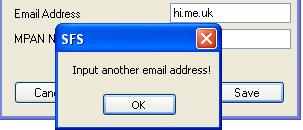
\includegraphics[scale=0.5]{test6dot2scrot}
		
		\subsubsection{Suppliers}
		
		If Suppliers is chosen, the add supplier form appears.
		
		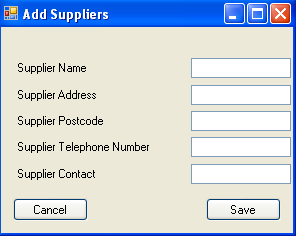
\includegraphics[scale=0.5]{frmAddSupplier_scrot}
		
		As above with the customer details, input the details, then click Save.  If there is an error in the details, the program will give an error message and data amendment is possible.  If there is no error and therefore the data insertion is successful, the save textbox will turn grey, signifying inactivity.
		
		Clicking the Cancel button will close the form, thereby not saving any of the data entered into the textboxes.
		
		Some things to note:
		
		\begin{itemize}
			\item{If there is no data to input into one textbox at the time of addition, input `NULL', do not just leave the textbox blank: doing so will display an error.}
			\item{UK telephone numbers must contain spaces between them, e.g. \textsl{01234 567890}, \textsc{NOT} \textsl{01234567890} or variants.}
			\item{The Supplier Contact textbox is the container for the name of the person who most frequently deals with communication with Sunny Future Solar at the supplier.  For example: Ben at Alternergy.}
		\end{itemize}
		
		\subsubsection{Components}
		
		If Components is chosen, the add component form appears.
		
		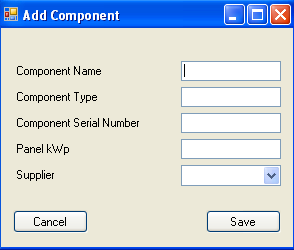
\includegraphics[scale=0.5]{frmAddComponent_scrot}
		
		Input the details, then click Save.  If there is an error in the details, the program will give an error message and data amendment is possible.  If there is no error and therefore the data insertion is successful, the save textbox will turn grey, signifying inactivity.
		
		Clicking the Cancel button will close the form, thereby not saving any of the data entered into the textboxes.
		
		Some things to note:
		
		\begin{itemize}
			\item{If there is no data to input into one textbox at the time of addition, input `NULL', do not just leave the textbox blank: doing so will display an error.}
			\item{The textbox labelled `Supplier' in this form should be used to specify which supplier supplies the added component.  If the supplier for the component does not exist at the time, it must be added before adding the component itself, using the supplier addition form documented above.}
		\end{itemize}
		
	\subsection{Removing customers, suppliers, or components}
	
	Sometimes, it may be necessary to permanently remove a customer, supplier, or component.  To do so, return to the main menu by pressing Close or Quit on several forms, or by logging in again, and click the `Remove' button, or Tab to it and hit Enter.  The form below is what is initially displayed.
		
	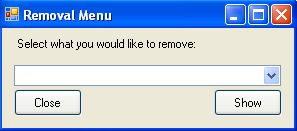
\includegraphics[scale=0.5]{frmRemove_scrot}
		
		\subsubsection{Customers}
		
		To remove a customer, select Customer from the drop down menu in `frmRemove', then select the appropriate customer in the form that appears and click `Remove', like in the example for removing the customer `Isabell Long'.
	
		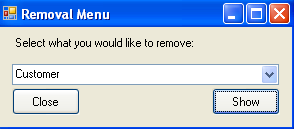
\includegraphics[scale=0.5]{customer-frmRemove_scrot}
		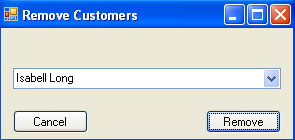
\includegraphics[scale=0.5]{customer-frmRemoveCustomer_scrot}
		
		To close the form after successful customer removal, click `Cancel'.
		
		\subsubsection{Suppliers}
		
		To remove a supplier, select Supplier from the drop down menu in `frmRemove', then select the appropriate supplier in the form that appears and click `Remove'.  If the supplier has components associated with it, it will not be removed and an error message will display.
		
		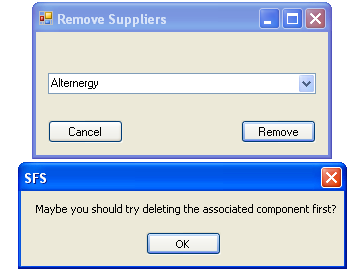
\includegraphics[scale=0.5]{test9dot2}
		
		To close the form after successful or unsuccessful supplier removal, click `Cancel'.
		
		\subsubsection{Components}
		
		To remove a component, select Component from the drop down menu in `frmRemove', then select the appropriate supplier in the form that appears and click `Remove', like in the example for removing the component `REC250'.
		
		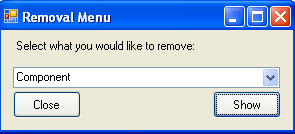
\includegraphics[scale=0.5]{component-frmRemove_scrot}
		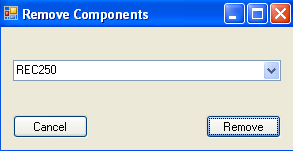
\includegraphics[scale=0.5]{component-frmRemoveComponent_scrot}
		
		To close the form after successful component removal, click `Cancel'.
		
	\subsection{Listing customers, suppliers, or components}
	
	It may be useful to list the contents of the database without having to delve into the database.  This can be done by clicking the List button on the main menu.  A window as in the screenshot below will appear.
	
	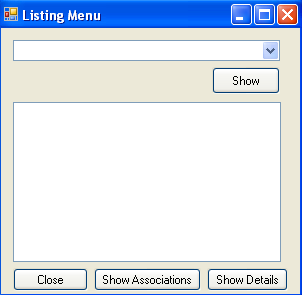
\includegraphics[scale=0.5]{frmList_scrot}
	
		There are many buttons at the bottom of this form: one to close the form, one to list the full details of the selected customer, and one to show any associations between customers, suppliers, or components.
		
		\textbf{Please note} that at present, the show associations button only works when component is selected, as it shows which supplier the component is supplied by.
		
	Upon clicking the button `Show Details' in the List form, a form will display that looks in the first instance like the screenshot below: this is where the full details of the selected customer\slash supplier\slash component will be shown.  This manual will delve into that a bit later on.
	
	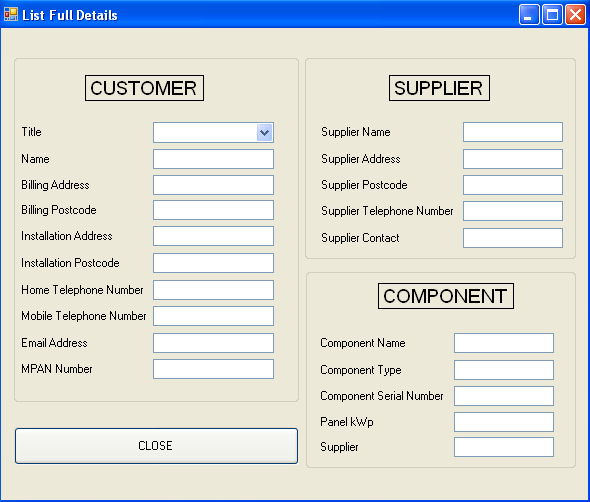
\includegraphics[scale=0.25]{frmListFullDetails_scrot}
	
		\subsubsection{Customers}
		
		To list customers, select Customers from the dropdown box.  Something akin to the following will display\footnotemark.
		
		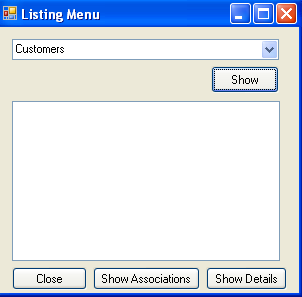
\includegraphics[scale=0.5]{customer-frmList-first_scrot}
		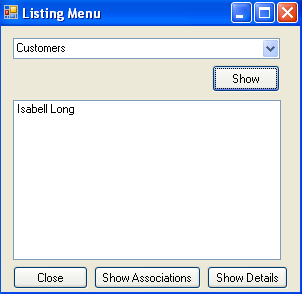
\includegraphics[scale=0.5]{customer-frmList-second_scrot}
		
		\footnotetext{In these examples, I have re-added the customer `Isabell Long' who was deleted earlier in the deletion explanations, for simplicity.}
		
		To search for a customer, enter a search term in the search box screenshoted below, and click Search.  The search results will display.
		
		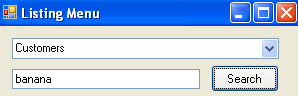
\includegraphics[scale=0.5]{searching_demo_scrot1}
		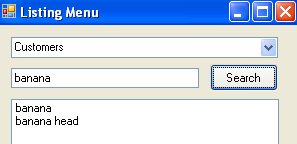
\includegraphics[scale=0.5]{searching_demo_scrot2}
		 
		To see the full customer details, click the `Show Details' button:
		
		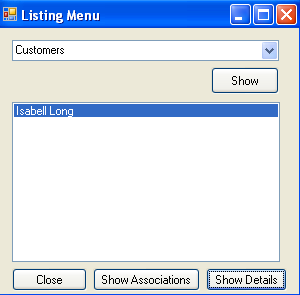
\includegraphics[scale=0.5]{customer-frmList-lfd_scrot}
		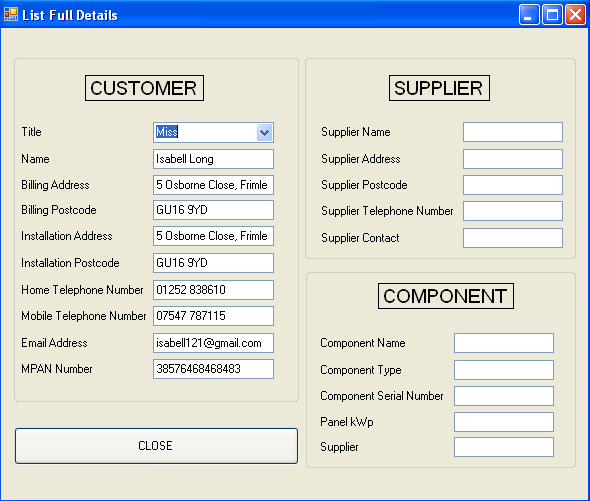
\includegraphics[scale=0.25]{customer-frmListFullDetails_scrot}
		
		The `Show Associations' button will show an error message if it is clicked anywhere but when `Components' is selected in the dropdown box.
		
		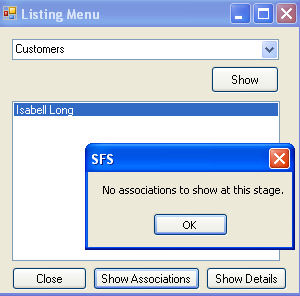
\includegraphics[scale=0.5]{customer-frmList-sa_scrot}
		
		\subsubsection{Suppliers}
		
		To list suppliers, select Suppliers from the dropdown box.  Something akin to the screenshot below will display\footnotemark.
		
		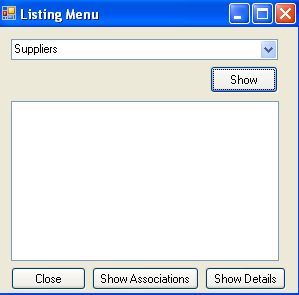
\includegraphics[scale=0.5]{supplier-frmList-first_scrot}
		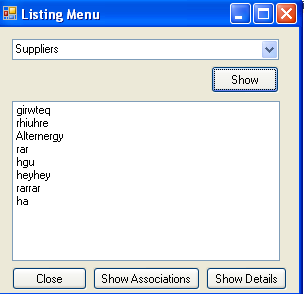
\includegraphics[scale=0.5]{supplier-frmList-second_scrot}
		
		\footnotetext{In these examples, I have re-added the supplier `Alternergy' that was deleted earlier in the deletion explanations, for simplicity.}
				
		To search for a supplier, enter a search term in the search box as screenshotted in the customer listing section.  The search results will display.
					
		To see the full supplier details, click the `Show Details' button:
		
		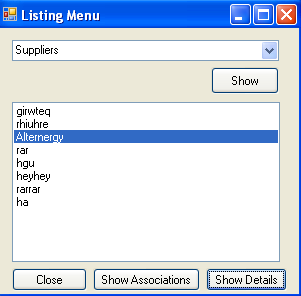
\includegraphics[scale=0.5]{supplier-frmList-lfd_scrot}
		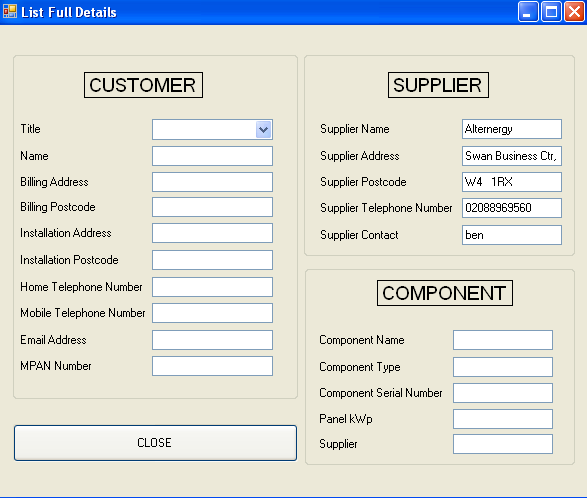
\includegraphics[scale=0.25]{supplier-frmListFullDetails_scrot}
		
		The `Show Associations' button will show an error message if it is clicked anywhere but when `Components' is selected in the dropdown box.
		
		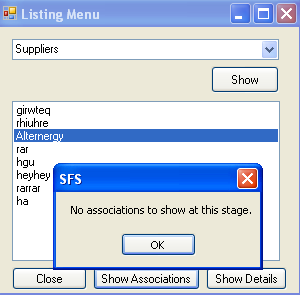
\includegraphics[scale=0.5]{supplier-frmList-sa_scrot}
		
		\subsubsection{Components}
		
		To list components, select Components from the dropdown box.  Something akin to the screenshot below will display.\footnotemark
		
		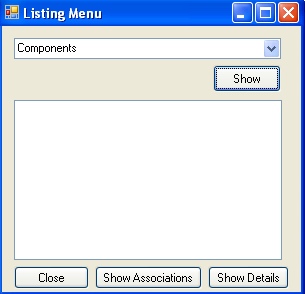
\includegraphics[scale=0.5]{component-frmList-first_scrot}
		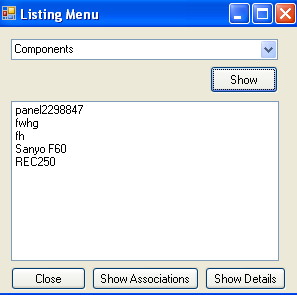
\includegraphics[scale=0.5]{component-frmList-second_scrot}
		
		\footnotetext{In these examples, I have re-added the component `REC250' that was deleted earlier in the deletion explanations, for simplicity.}
		
		To search for a component, enter a search term in the search box as screenshoted in the customer listing section, and click Search.  The search results will display.
		
		To see the full component details, click the `Show Details' button.
		
		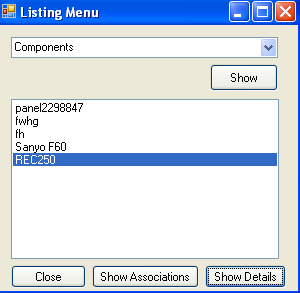
\includegraphics[scale=0.5]{component-frmList-lfd_scrot}
		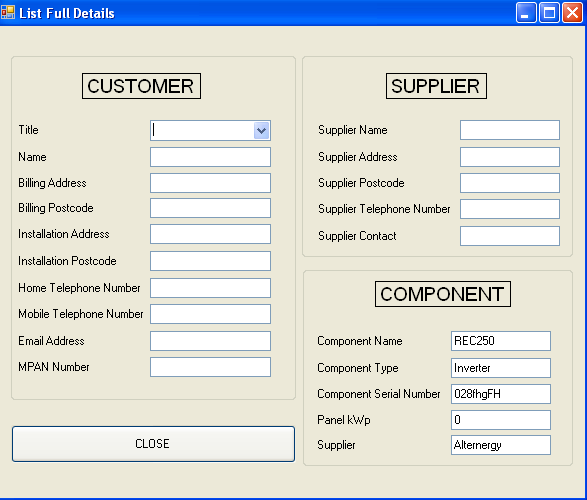
\includegraphics[scale=0.25]{component-frmListFullDetails_scrot}
		
		Now the `Show Associations' button will not display an error message!  Clicking that button when the selected component is `REC250' will display that the component is supplied by `Alternergy', and so on.
		
		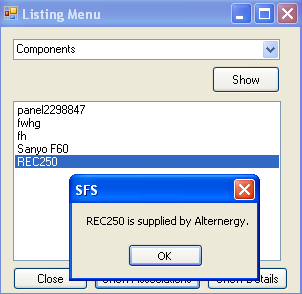
\includegraphics[scale=0.5]{component-frmList-sa_scrot}
		
	\subsection{Reports}
	
	Reports can be produced for various things using this system: logs, quotes, invoices, and surveys.  To access the reports menu, click Reports from the main menu; the form shown should appear.
	
	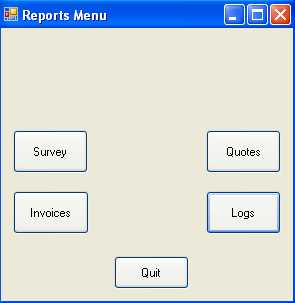
\includegraphics[scale=0.5]{frmReportMenu_scrot}
	
		\subsubsection{The log forms}
		
		Clicking `Logs' will open a screen like the one below.
		
		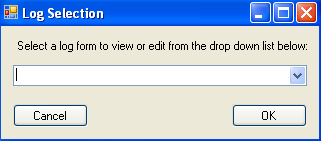
\includegraphics[scale=0.5]{frmReportLog_scrot}
		
		Select a month\slash year from the drop down menu, and click OK.  This will open the log form for the selected month and year in Microsoft Word, which you can edit and save.  Close the Word document to return to the program, or just click the program window on the task bar.  See the screenshots for an example of the log form from December 2011.
	
	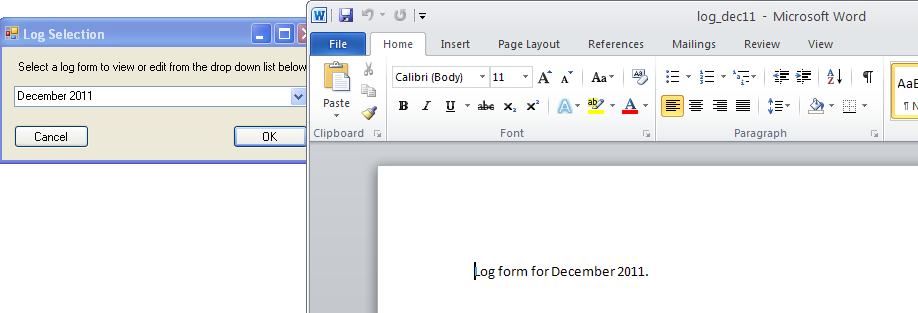
\includegraphics[scale=0.5]{log-dec11-select-word_scrot}
	
		\subsubsection{The quotations}
		
		Currently, the quotations only automate inputting of the billing address, however they are still useful.  To open a quotation in Microsoft Word, click `Quotes' in the report menu and select a customer to open the quote for.  An example is below.
		
		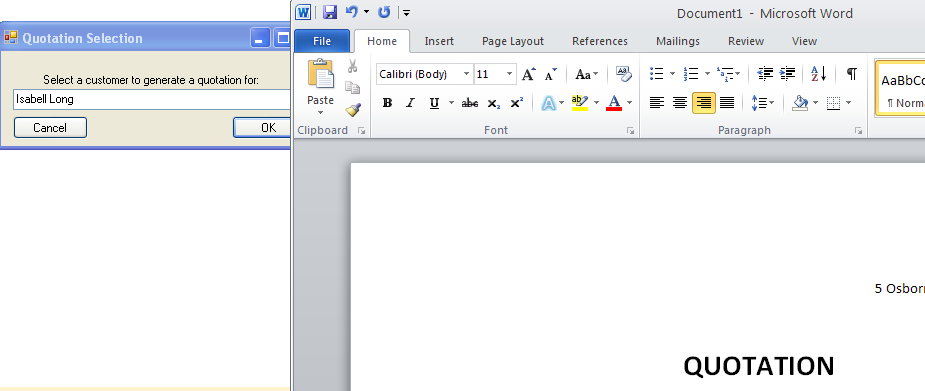
\includegraphics[scale=0.5]{quote-IL-select-word_scrot}
		
		\subsubsection{The invoices}
		
		Currently, the invoices only automate inputting of the billing address, however they are still useful.  To open an invoice in Microsoft Word, click `Invoices' in the report menu and select a customer to open the invoice for.
		
		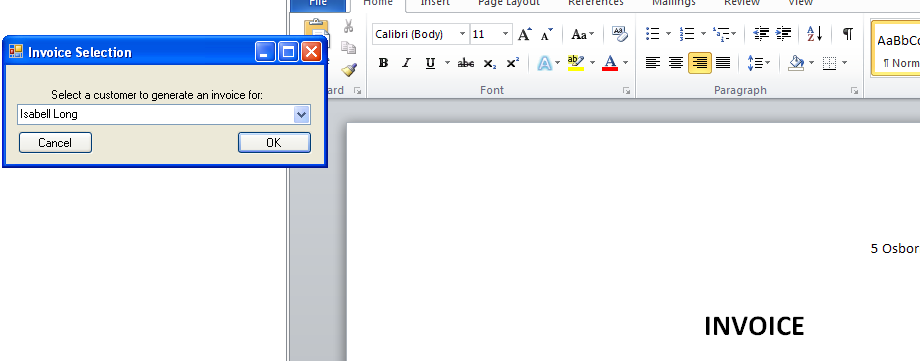
\includegraphics[scale=0.5]{invoice-IL-select-word_scrot}
		
		\subsubsection{The surveys}
		
		Currently, the surveys only display the customer details, and no other details can be added.  To view the surveys, click the `Surveys' button in the report menu and select a customer to open the survey for.

		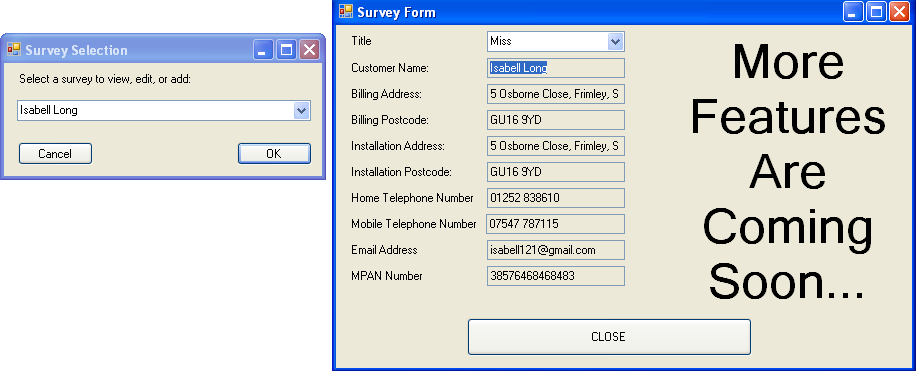
\includegraphics[scale=0.25]{survey-IL-select_scrot}

	\subsection{Error handling}
			\begin{longtable} { | p{6cm} | p{6cm} | }
		\hline
		\textbf{Error text} & \textbf{Recovery}\\
		\endfirsthead		
		\hline
		\textbf{Error text (cont.)} & \textbf{Recovery (cont.)}\\
		\endhead
		\hline
		``Incorrect username or password.  Try again.'' & An incorrect username or password, or both, has been entered.  Click `OK' and re-enter the login details.\\
		\hline
		``Input a valid email address!'' & You most likely did not include an @ symbol in the entered email address---maybe you were on a US keyboard and entered a '' instead?  Click `OK' and reenter the email address in its entirety, properly.\\
		\hline
		``There has been an error.'' & One or more of the textboxes\slash dropdowns were blank, most likely.  Click OK and make sure that all the textboxes have something in them, even `NULL' for on-purpose values that do not have information for, then click Save again.\\
		\hline
		``This window will close and these details will not be saved.'' & Self-explanatory.  Click the `OK' button to close the window without saving the details that may or may not have been entered.\\
		\hline
		``Enter a value in each of the boxes, and make it a valid one!'' & Not all the textboxes have been populated with data.  Populate them, even with ``NULL'', then click `Save' again.\\
		\hline
		``No associations to show at this stage.'' & Informational.  Click `OK' to dismiss the box.\\
		\hline
		``Cannot show associations; please select an item from the list.'' & The program cannot show the associated supplier for the component because no component has been selected.  Click `OK' to dismiss this box, select a supplier, then reclick `Show Associations'.\\
		\hline
		``Select a customer to generate an invoice for!'' & This appears because no customer has been selected from the dropdown box at the top of the form from whose details an invoice can be generated.  Click the dropdown box and select a customer, after having dismissed the error message, then redisplay the invoice.\\
		\hline
		``No form was selected.'' & No log form was selected from the dropdown box.  Click `OK' to dismiss the error message, then actually select a log form to open from the list and click `OK' on the selection form.\\
		\hline
		``Data insertion failed.'' & Self-explanatory.  Click `OK' to dismiss the error and re-enter whichever information was not included or was in the wrong format.\\
		\hline
	\end{longtable}
